\clearpage
%% temporary titles
% command to provide stretchy vertical space in proportion
\newcommand\nbvspace[1][3]{\vspace*{\stretch{#1}}}
% allow some slack to avoid under/overfull boxes
\newcommand\nbstretchyspace{\spaceskip0.5em plus 0.25em minus 0.25em}
% To improve spacing on titlepages
\newcommand{\nbtitlestretch}{\spaceskip0.6em}
\pagestyle{empty}
\begin{center}
\bfseries
\nbvspace[1]
\Huge
{\nbtitlestretch\huge
אלגוריתמים מבוזרים בגרפים\\
236610}

\nbvspace[1]
\normalsize

סיכום זה נכתב על בסיס ההרצאות והמצגות של פרופ. חבר קרן צנזור-הלל כפי שהוצגו במסגרת הקורס "אלגוריתמים מבוזרים בגרפים" 236610 שניתן במהלך סמסטר אביב 2018 בפקולטה למדעי המחשב בטכניון.\\
\nbvspace[1]
\small נכתב ונערך ע"י\\
\normalsize אלעד נחמיאס\\[1.5em]
\footnotesize אם מצאת במסמך טעויות, אי-דיוקים, חוסרים או שברצונך להציע הצעות לשיפור, אנא צור איתי קשר: eladnah@gmail.com

\nbvspace[2]

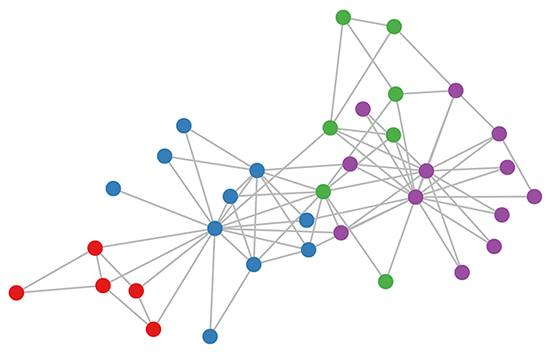
\includegraphics[width=3.5in]{./graphics/cover.jpg}
\nbvspace[3]
\normalsize

\textsuperscript{\faCopyright} כל הזכויות שמורות\\
\large
הפקולטה למדעי המחשב בטכניון
\nbvspace[1]
\end{center}
\pagebreak
